\documentclass{mcmthesis}
\mcmsetup{CTeX =false,   % 使用 CTeX 套装时,设置为 true
        , problem = 8,
        sheet = true, titleinsheet =true, keywordsinsheet = true,
        titlepage =false, abstract = false}
\usepackage{palatino}
\usepackage{lipsum}

\usepackage{geometry}
%===============设置正文和数学字体=============================
%有些字体需要安装一些字体文件,注意辨别。
%我参照 MCM论文集的字体 使用如下宏包来定制字体。

\usepackage{graphicx}
\usepackage{subfigure}
%设置段落之间的距离,若不需要删除或者注释掉即可。
\setlength\parskip{.5\baselineskip}
\newtheorem{definition}{Definition}[section]
%\def\abstractname{Summary}%可修改摘要名称

\usepackage{indentfirst}
\setlength{\parindent}{2em}

\usepackage{chngpage}
\usepackage{array}
\usepackage{booktabs}
\usepackage{threeparttable}
\usepackage{longtable}
\usepackage[numbers,sort&compress]{natbib}
%%% 实现参考文献标号在右上角
\newcommand{\upcite}[1]{\textsuperscript{\textsuperscript{\cite{#1}}}}
%然后引用的时候使用\upcite{}的格式(一般的正常引用格式为\cite{})

\usepackage{titletoc}
\titlecontents{section}[3cm]{\bf \large}{\contentslabel{2.8em}}{}{%
\titlerule*[0.5pc]{$\cdot$}\contentspage}%
\titlecontents{subsection}[4cm]{\normalsize}{\contentslabel{2.5em}}{}{%
\titlerule*[0.5pc]{$\cdot$}\contentspage}%
\titlecontents{subsubsection}[5.3cm]{\normalsize}{\contentslabel{3.0em}}{}{%
\titlerule*[0.5pc]{$\cdot$}\contentspage}%

\title{\large Optimal Control of a Linear Discrete System}
\author{Dazheng Fang//Haorui li//Yao Yao//Zhiyi Shi }


\date{\today}

\geometry{left=3.0cm,right=3.0cm}

\begin{document}


\begin{abstract}

In the real world, many real systems are time-discrete in nature.Even if the system is time-continuous, because the computer is based on such discrete digital technology as time and value, the implementation of computer control must be treated as a discrete system after time discretization.Therefore, it is necessary to discuss the optimal control of discrete time systems.

First of all, We build up the mathematical programming model of the optimal control problem from the conditions of the dynamic equation.
%通过Lagrange乘子法将等式约束下的极值问题化为无约束的极值问题,使用离散的欧拉方程进行限制,到达下确界。迭代法求出X(T)和C的关系。并使用X(T)的范围求出C的范围。再在C的取值范围中,求得最优解。
For the problem(2), first,  using the Lagrange undetermined multiplier method change the extremum problems with equality constraints(ECEP) into an unconstrained extremum problem(EP). Second, using discrete Euler-Equations to restrict variables and reach the lower bound. Third, using iteration method to get the relationship of $X(T)$ and C, then figure out their  ranges. Finally, searching in the value range of C to get the optimum point.%%%%%%%%%%%%MATLAB!!!!%%%%%%%
%UNCHANGED!!!!!!!!!!!!!!!!!!!!!!!!!!!!!!


Finally, based on the theory of the traditional VRP (Vehicle Routing Problem), taking the shortest time and lowest risk and low economic losses as the total constraint conditions, considering the road carrying capacity constraints, refuge capacity, garage capacity constraint conditions and so on, according to the category and the landing site of the hurricane, the comprehensive evacuation planning model is established. The processing conditions under the category 1-5 hurricane conditions are simulated, and the shortest time is obtained under the model condition, which is the shortest release time before the hurricane.
%%%%%%%%%%%%%%%%%%%%%%%%%%%%%%%%%%%%%%%%%%%%%%

\begin{keywords}
Lagrangian Multiplier Method ; Euler Equations; 
\end{keywords}
\end{abstract}
\maketitle
%\pagestyle{empty}
\newpage                                                          %
%==================================================================
%====================生=成=目=录===================================
\begin{adjustwidth}{-1cm}{0cm}

\setcounter{tocdepth}{3}
\thispagestyle{empty}
\tableofcontents                                                  %

\end{adjustwidth}


\newpage

\pagestyle{fancy}

\setcounter{page}{1}
\section{Introduction}
\subsection{Background}

In the real world, many real systems are time-discrete in nature.Even if the system is time-continuous, because the computer is based on such discrete digital technology as time and value, the implementation of computer control must be treated as a discrete system after time discretization.\cite{journals/kybernetika/StechaKKL73}

Therefore, it is necessary to discuss the optimal control of discrete time systems.


\subsection{Problem Restatement}

Suppose that we have a discrete-time linear system with the following dynamic equation:

$$\begin{array}{l}
x(k+1)=A x(k)+B u(k) \\
\end{array}$$

where x(t) is the state variable at time t; u(t) is control variable at time t; A is the state matrix; and B is the control matrix. Suppose that the initial state x(0) is known. Demine the control series u(t), t=0, 1, …, T, such that the state at the end of the time horizon x(T) falls in a predetermined interval and the energy consumed in the entire time horizon (which can be captured by the weighted summation of the magnitude square of controls over time) can be minimized. The values of the controls have upper bounds.

And the six problems are:

(1)	Develop the mathematical programming model of the optimal control problem.

(2)	Set up the scale of the problem (i.e., the dimension of the state vector and the control vector) by yourself, as well as the values of the matrices A and B, the initial state and the upper bounds of the controls. Solve the problem by using the tools in Matlab and obtain the optimal control policy.

(3)	Change the value of A and analyze its impact on the controls and the objective function.

(4)	Change the upper bounds of the controls and analyze their impact on the controls and the objective function.

(5)	Change the length of the time horizon (i.e., the value of T) and analyze its impact on the controls and the objective function.

(6)	Write a research report, which must include the description of the problem, definition of the notations, explanation of the data, mathematical formulation of the problem, method of solving the problem, analysis of the result, conclusion, and references. The source code must be submitted.


\subsection{Our Work}

TO BE DOWN

\section{List of Notation}

\begin{center}
\begin{longtable}{p{.1\textwidth}p{.8\textwidth}m{.4\textwidth}}
\caption{The List of Notation}\\
\hline
Symbol& Meaning \\
\hline

$J$      & System performance index, optimization function
                                                         \\
$\bar J$ & Loss function    \\
$L_k$      & The increment of performance indicator J in the Kth sampling period
                                                          \\
$\lambda$     & Lagrangian multiplier matrix
                                                                                        \\ \hline

 \end{longtable}
 \end{center}


\section{Problem One: Build up the Model}
From the problem we define the system performance index, in other words, optimization functio J as:
%%%%%%%%%要不要加权?%%%%%%%%%%
$$J=\frac{1}{2}\sum^{T-1}_{k=0}u^T(k)u(k)$$

$Notes$ : Now the weight of every step is 1

The problem can be rewriten as:
\begin{align}
min & \text{ } J=\frac{1}{2}\sum^{T-1}_{k=0}u^T(k)u(k)\\
S.t. \text{ }& x(k+1)=A x(k)+B u(k)\\ &  k < T\\& k \in Z^+    
\end{align}

By Lagrange undetermined multiplier method we can get:
$$\bar J=\sum^{T-1}_{k=0}\{\frac{1}{2}u^T(k)u(k)+\lambda(k+1)[-x(k+1)+Ax(k)+Bu(k)]\}$$

And this is the loss function.

Define the increment of performance indicator J in the Kth sampling period as:
$$L_k=\frac{1}{2}u^T(k)u(k)+\lambda(k+1)[-x(k+1)+Ax(k)+Bu(k)]$$

Step backward:
$$L_{k-1}=\frac{1}{2}u^T(k-1)u(k-1)+\lambda(k)[-x(k)+Ax(k-1)+Bu(k-1)]$$

Then solve the  derivation:
\begin{equation}\begin{array}{l}
\frac{\partial L_{k}}{\partial x(k)}=A^{T} \lambda^{T}(k+1) \\\\
\frac{\partial L_{k}}{\partial x(k)}=-\lambda^{T}(k) \\\\
\frac{\partial L_{k}}{\partial u(k)}=u(k)+B^{T} \lambda^{T}(k+1) \\\\
\frac{\partial L_{k}}{\partial u(k)}=0
\end{array}\end{equation}

By using Euler equation, we will have:

$$\begin{cases} A^T\lambda^T(k+1) =\lambda^T(k) \\u(k)+B^T\lambda^T(k+1)=0 \end{cases}$$

Let$\lambda^T(1)=C$, therefore:

 $$\lambda^T(k)=(A^T)^{-(k-1)}C$$

$$u(k)=-B^T(A^T)^{-k}C$$

We can easily see that

$$x(k+1)=Ax(k)-BB^T(A^T)^{-k}C$$

Thus:

\begin{align}
&x(1)=A x(0)-B B^{T} C \\
&x(2)=A^{2} x(0)-A B B^{T} C-B B^{T}\left(A^{T}\right)^{-1} C \\
&x(3)=A^{3} x(0)-A^{2} B B^{T} C-A B B^{T}\left(A^{T}\right)^{-1} C-B B^{T}\left(A^{T}\right)^{-2} C \\
\cdots \\
& x(k+1)=A^{k+1} x(0)-\sum_{i=0}^{k} A^{k-i} B B^{T}\left(A^{T}\right)^{-i} C
\end{align}


\section{Problem Two: Solve the problem using MATLAB tool}

The demand distribution defines the number of people arriving at the station nodes during the evacuation process. The demand distribution depends on the potential population of the evacuation area depending on the transport system. This demand not only has spatial dependence, but also has time dependence. To determine how many evacuees will arrive at each station node, we need to define a service area to determine its appeal scope. One way to do this is to use the concept of the Thiessen Polygon \cite{Bretschneider2011A}. The Thiessen Polygon is centered around the station node and the nearest family is located in the same service area. By dividing the network into a number of adjacent polygons, families are assigned to the Thiessen Polygon where their nearest assembly point is located.

In the study, we determined the potential demand by using the Thiessen Polygon to determine the service area of the station node. Due to the evacuees in the evacuation process, the demand of the station nodes is uncertain, mainly manifested in the following two situations:

\begin{itemize}

\item Those who have been registered to evacuate will change their minds and evacuate by private cars or other means, reducing the need for evacuation;
\item Personnel who have not been registered prepare to evacuate, including tourists or travel agents, and increase evacuation demand.

\end{itemize}

The demand distribution in this paper is based on the pre-population survey data covered by the station node, assuming that it is subject to uniform distribution. For example, if the number of evacuees covered by the survey is 40, then U [30, 50], and the demand will be gradually generated according to the Mobilization Curve.
For station nodes, assuming that they have a certain storage capacity, the evacuees can wait for a while before they evacuate. Emergency evacuation in practice, can under the circumstances of road network, through the whole evacuation phases to define the generated during evacuation demands, in order to make every vehicle evacuation route.

Goerigk proposed the mobilization curve \cite{Goerigk2014A,Goerigk2013Branch}, also known as the S type curve, used to estimate demand in different time evacuees percentage. In the event of natural disasters, the cumulative percentage of evacuation demand can be calculated by the time-varying curve function. The time-varying curve is expressed as follows:


\begin{equation}\label{1}
C(t) = \frac{1}{{(1 + {e^{ - \alpha (t - h)}})}}
\end{equation}

\begin{equation}\label{2}
C(0) = 0
\end{equation}

Where:

$C(t)$ is the cumulative percentage of withdrawal demands from time to time;

$a$ is the loading rate or the reaction rate of the public to the evacuation instructions, also expressed as the slope of the time curve;

$h$ is the time required for half of the demand in the system;

$t$=0 represents the time the evacuation order is released.

The individual loading time is the time when they arrive at the station node. $h$ can be determined according to the peak value of the departure time of the traffic or half of the estimated allowable evacuation time. Choose half the load time as an input parameter for the system. If time varying curve is used to calculate the cumulative percentage of the traffic demand is loaded into the road network, then according to the nature of the disaster, we can use different half load time to impact load parameter. therefore, in the process of evacuation, the choice of half load time is crucial~\cite{Sayyady2010Optimizing,So2010Managing}.

Loading time usually includes departure time and time required to reach the station node. Departure time refers to the time each person spends preparing for withdrawal once the evacuation order is released. Through this definition, we can know that the loading time varies based on the type of events, the relative severity of events, the communication efficiency of the public and the involvement of emergency management centres.

In the study of this paper, we do not cover the departure time, but only the time that needs to reach the station node.

By introducing different loading rates during the implementation phase of the evacuation plan, the withdrawal situation will change.

In the case of low loading rates usually, more people are responding to instructions in the early stages of evacuation, while the high loading rate, a large number of evacuees spend a lot of time preparing for the evacuation.

In the case of low loading rate, people gradually reach the station node within the time range of evacuation, but for the high loading rate, a large number of people rush to the station node during the final phase of evacuation,as is shown in Figure ~\ref{fig:2}.

\begin{figure}[htbp]
  \centering
 
  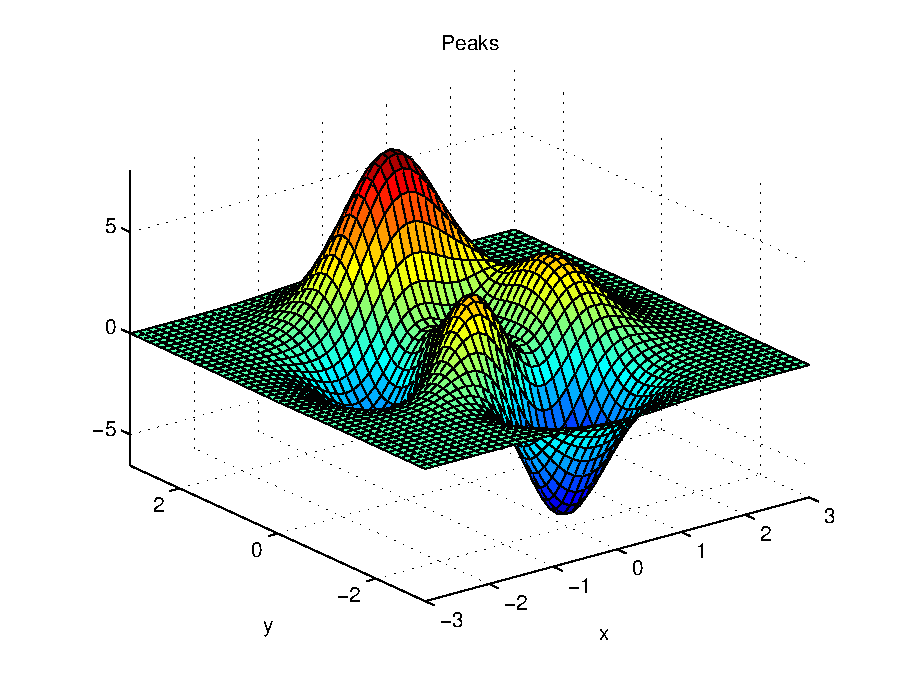
\includegraphics[width=0.7\textwidth]{./picture/figure2.eps}
  \caption{Behavioral Response Curves}\label{fig:2}
 \end{figure}

In the case of a hurricane, the initial phase of withdrawal is usually slow, and the demand for station nodes is not greater than the capacity of the vehicle. But in the final phase of the evacuation, the demand may be concentrated, and the cumulative result is that the demand for a station node is greater than the capacity of the vehicle. At this moment, we need  to send vehicles from another station node to meet their needs, carrying away for the rest. With the demand of the other station node considering again, a reasonable, optimizing transportation route can be arranged.

\section{The Comprehensive Evacuation Planning Model}
\subsection{Model Preparation}

\begin{itemize}

\item Station nodes: In this problem, the locations of all station nodes are known and fixed, and the demand generation changes over time to meet the S type behavior curve. Requirements may exceed the load capacity of the vehicle during the process of time change. In this case, it may be necessary to mobilize the vehicle from other station nodes or carry out the second transport. Having no time limit on the vehicle service, evacuees can be carried out at any time in station nodes, and the transport vehicle is set at the set point;
\item Transport vehicle: In this problem, all vehicles start from the shelter, via the station node, and then complete the transport mission, during which the overload operation is not allowed to exceed the maximum driving time of the vehicle;

\item Shelter: In this problem, there are several shelters whose location and capacity have been determined.
\end{itemize}

VRP \cite{Dikas2016Solving,He2015Model} generally defined as: on a range of clients point (location known or can be estimated) in satisfying certain constraints (such as the demand for goods, the delivery time of delivery, the vehicle capacity constraints, etc.), reasonably arrange the vehicle distribution route, making the vehicle through them in an orderly way to achieve a certain goal (such as the shortest mileage and least cost, least time, use as little as possible and so on). The representation of VPR can be seen in Figure 3.

\begin{figure}[tbp]
  \centering{
  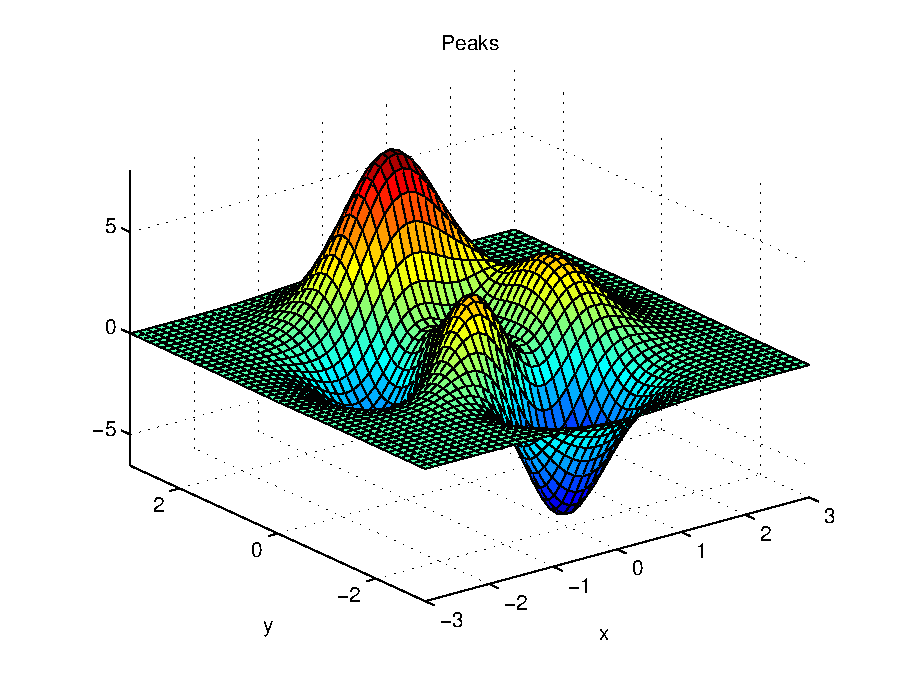
\includegraphics[width=0.7\textwidth]{./picture/figure3.eps}}
  \caption{A Typical Vehicle Routing Problem}\label{Figure3}
\end{figure}

Based on the traditional VRP, a comprehensive evacuation planning model is established to satisfy the constraint conditions:
\begin{itemize}
  \item Time constraint: the total withdrawal time is the shortest in the case of meeting all the evacuees' needs and not violating the constraints;
  \item Risk constraint: minimum risk of meeting the minimum evacuation time;
  \item Carrying capacity constraint: the number of customers on each vehicle path is limited no more than a constant;
  \item Road afford ability constraint: the total carrying capacity on the road is not allowed to exceed the road capacity;
  \item Shelter capacity constraint: the total population in the shelter shall is not allowed to exceed the capacity limit;
  \item Priority relationship constraints: the more endangered areas have priority access;
  \item Path first constraint: after every vehicle completes its mission, records its shelter and the time to reach the sanctuary, preparing for the assignment of the next mission.
\end{itemize}

Before each task, we need to update the network node demand, shelter of residual capacity and the starting position of the vehicles, where each task should be according to the last mission at the end of the vehicle at the beginning of status to the caller, get the transport vehicles in the task.

\subsection{Modeling}

We now describe an optimization model that includes the assumptions of the previous section %%\cite{Goerigk2014Combining}.

The considered time horizon is denoted by $T$. This is not the evacuation time we are aiming for, but an upper bound on the evacuation time that is needed by our model. This quantity is used to build the time expanded network.

For public transportation we assume that there is already an established set of collection points, where evacuees gather for further transportation to shelters. For each collection point it is known how many people will appear at this point in each time step. We also given a set of possible shelter location. For each such location we are given the number of people ${W_j}$ that this shelter can hold and additionally the parking space ${C_j}$ available near this shelter.

The set of buses available for the public evacuation transit is denoted by B. For simplicity, we assume that all buses have the same capacity ${N_0}$ (however, different capacities can easily be included in our model). Besides all cars carry the same number of people.

Once the used shelter locations have been chosen, the public and private traffic will pour into the shelter. The private traffic is modeled as a dynamic network flow, the public traffic (the buses) as a dynamic multi commodity network flow. The private traffic is a single commodity whereas each bus is a commodity of its own. The flow of the buses has to be chosen such that all people that need public transportation can be brought to shelter locations while respecting the bus capacity. Both flows are chosen simultaneously in a system optimal way.

The total risk exposure is given by the sum of the risks of the individual arcs over all time steps. The risk of a single arc at a time step is given by the risk value of the arc multiplied with the number of people on this arc at this time step.

Formulating these aspects mathematically, we propose the following multi-criteria mixed-integer programming model, which we call the Comprehensive Evacuation Problem (CEP)\cite{Murray2013Evacuation,Ng2015Sharp,Ng2010Reliable}

In this mixed integer program we use the following variables: $\delta _{ij}$ denotes traversal of arc (i,j) $ \in $ A. $x_{ij}^t$ denotes the spend time passing arc (i,j). $r_{ij}^t$ denotes the risk factor passing arc (i,j) at time $t$. $f_{ij}^t$ denotes the number of evacuees using cars passing arc (i,j) at time $t$. In contrast, $g_{ij}^t$ denotes the number of evacuees using bus $b$ to go from node $i$ to node $j$ at time $t$. $\eta $ represents the jam factor, which depends on the magnitude of the hurricane, the location of the landing, and the average number of evacuees passing arc (i,j) at time $t$. $B_{ij}^t$ denotes the number of bus driving on arc (i,j) at time $t$.In the same way, $C_{ij}^t$ denotes the number of car driving on arc (i,j) at time $t$. $P_j^t$  denotes the number of people in the $j$ shelter at time $t$. $r$ denotes the capacity factor.


\begin{equation}\label{3}
\Delta \min (\Delta ,R)
\end{equation}

\begin{equation}\label{4}
\Delta  \ge (2n - 1) \times \max (\sum\limits_{(i,j) \in A} {\sum\limits_{t \in T} {\delta _{ij}^tx_{ij}^t} } ) + \Delta t
\end{equation}

The objective (1) is to minimize the evacuation time $\Delta $ and the risk $R$ ,These objectives are computed using constraints (2)-(4). Constraints (2) ensure that $\Delta $ is the maximal evacuation time. The risk $R$ depends on the number of people passing a link. This relation is expressed in constraint (3)and(4).

\begin{equation}\label{5}
 R = \sum\limits_{(i,j) \in A} {\sum\limits_{t \in T} {r_{ij}^t} } (f_{ij}^t + \sum\limits_{(i,j) \in A} {{\rm{g}}_{ij}^t} ) + W + V
\end{equation}

\begin{equation}\label{6}
\sum\limits_{(i,j) \in A} {\sum\limits_{t \in T} {f_{ij}^t} }  = {N_i} \times a\%
\end{equation}

\begin{equation}\label{7}
n = \left[ {\frac{{{N_{\rm{i}}} \times (1 - a\% )}}{{{B_i} \times {N_0}}}} \right]{\rm{ + }}1
\end{equation}

\begin{equation}\label{8}
x_{ij}^t = \eta \frac{{{S_{ij}}}}{{{v_b}}}
\end{equation}

\begin{equation}\label{9}
{\rm{g}}_{ij}^t = {N_0} \times B_{ij}^t
\end{equation}

\begin{equation}\label{10}
C_{ij}^t{\rm{ = p}} \times {{\rm{C}}_i}
\end{equation}

In the equation (5), $n$ means the number of journeys that the bus needs to transport, and the calculation should Integer plus one. Equation (8) - (10) is the road traffic that is used to constrain not to exceed its maximum capacity at time $t$.

\begin{equation}\label{11}
B_{ij}^t = {\rm{p}} \times {{\rm{B}}_i}
\end{equation}

\begin{equation}\label{12}
C_{ij}^t + B_{ij}^t \le {V_{ij}}
\end{equation}

The individual and the public traffic are linked together in the edge capacity constraints (11)-(12). Each used shelter must supply enough parking space and enough room to support evacuees.

\begin{equation}\label{13}
C_j^t \le {C_j}
\end{equation}

\begin{equation}\label{14}
P_j^t \le r{W_j}
\end{equation}

\begin{equation}\label{15}
r = \frac{{{N_{\rm{i}}}}}{{{W_j}}}
\end{equation}

When a hurricane is stronger, it may require a massive evacuation, that is, to consider the interaction of the three states. The site selection, risk coefficient, road congestion, and site accommodation will be affected, we need to reset the influence parameters to get the minimum required time and the site situation again.

Optimization method: When the forecast hat hurricane level is high, we can arrange inland evacuation ahead, in the case of ensure the overall time is enough for the coastal areas to evacuate to the site of the corresponding time calculation.

Advantage: Inland remove first can reduce the road pressure; Coastal remove later can increase the economic benefit.Compare the results again and get the final optimization plan.

\subsection{Model Solution}
Based on the above model and the parameters involved in the model, the final evacuation time is obtained by programming, and the result is shown in the table below:
\begin{table}[!htb]
\centering
\setlength{\abovecaptionskip}{0pt}%    
\setlength{\belowcaptionskip}{10pt}%
\caption{The Evacuation time}
\begin{tabular}{ccccccc}
\toprule[1.5pt]
Hurricane level &1&2&3&4&5&6\\
Evacuation time &11.4&18.2&24.28&33.6&47.8&49.6\\
\bottomrule[1.5pt]
\end{tabular}
\end{table}
%\begin{figure}[h]
%  \centering{
%  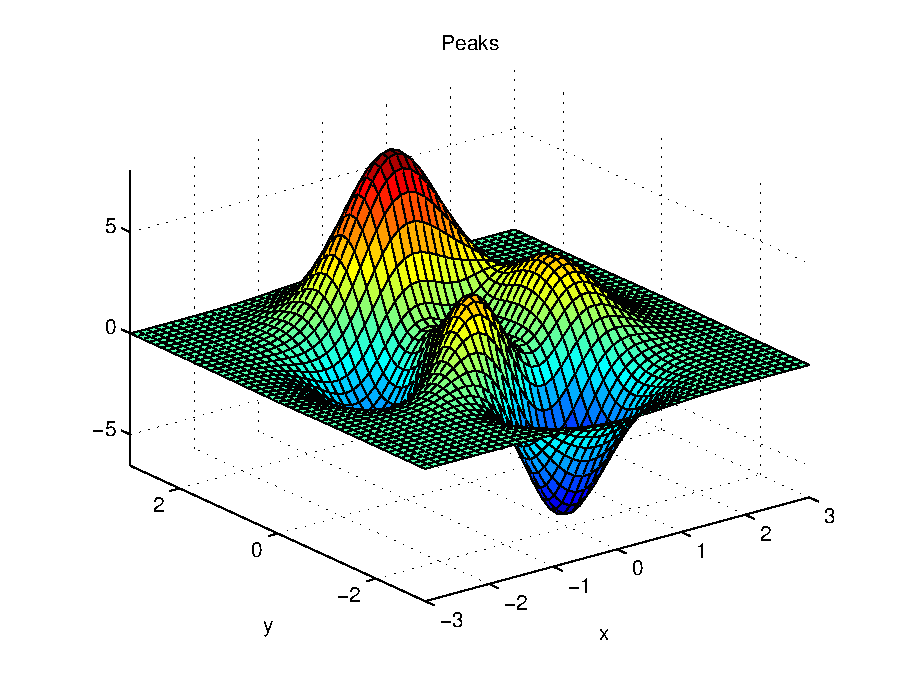
\includegraphics[width=0.7\textwidth]{./picture/figure4.eps}}
%  \caption{The Evacuation Time}\label{Table1}
%\end{figure}



As shown in the figure above, it is necessary to calculate the time required for a category 1- 5 hurricane, including the withdrawal time required for the optimization programme.

Because the evacuation and time of personnel also satisfied the curve of $S$ type curve, it can be used to draw the time-varying personnel evacuation curve of hurricane from category 1 - 5, which can be seen in figure4.

\begin{figure}[h]
  \centering{
  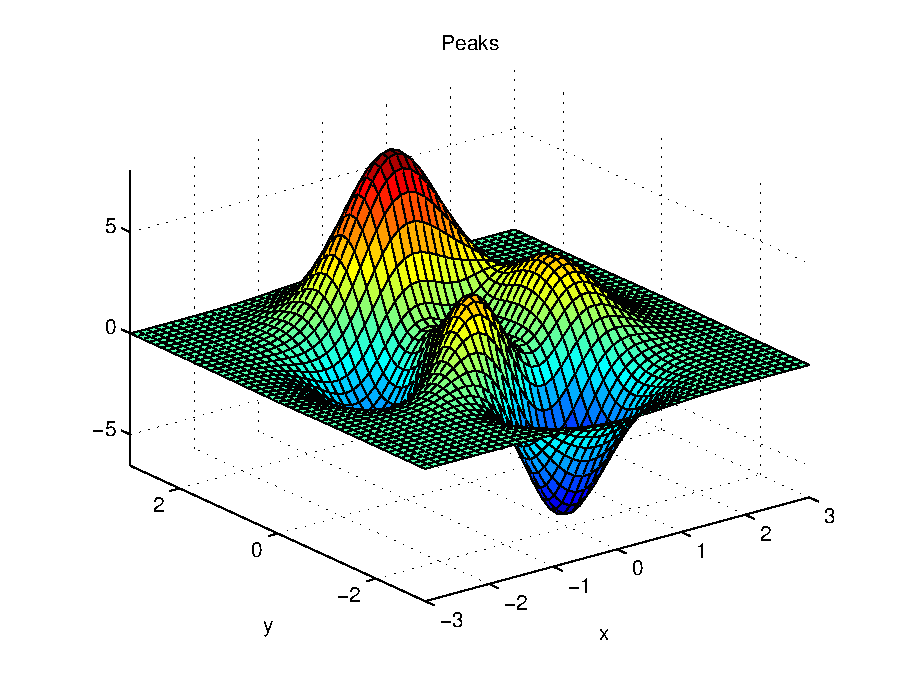
\includegraphics[width=0.7\textwidth]{./picture/figure5.eps}}
  \caption{The time-varying personnel evacuation curve of hurricane from category 1 - 5}\label{figure4}
\end{figure}

On the basis of guarantee the safety of life, we put forward the optimization scheme, when hurricane prediction level too high, let let evacuated inland areas, in order to improve the economic benefit of coastal, and reduce economic loss. The maximum population density due to coastal areas, and abide by the $S$ type curve evacuation rules.

\begin{figure}[h]
  \centering{
  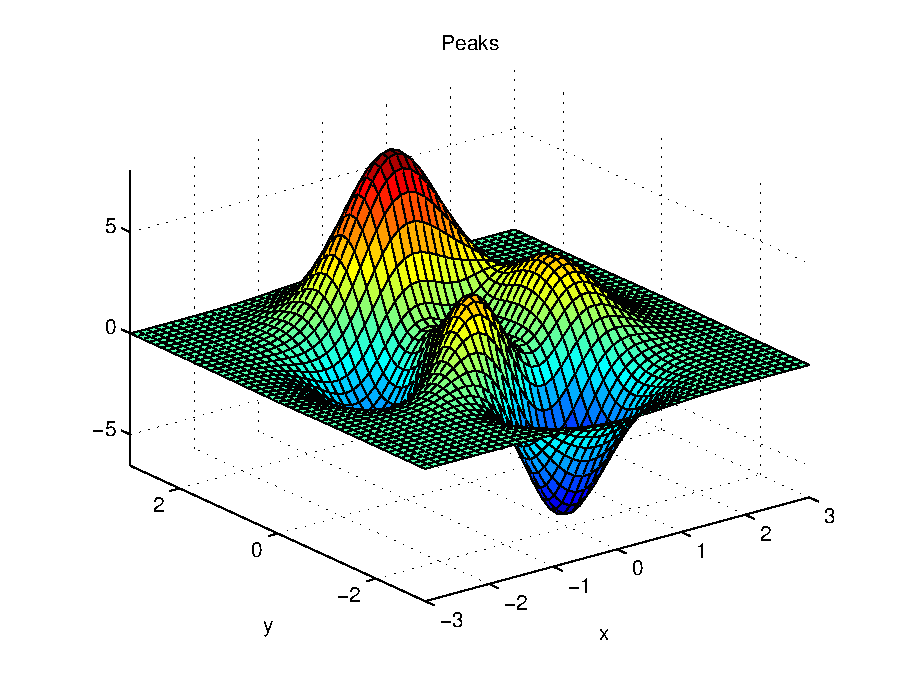
\includegraphics[width=0.7\textwidth]{./picture/figure6.eps}}
  \caption{Optimize personnel evacuation curve}\label{figure5}
\end{figure}

Under the same Five - level hurricane conditions, the optimization scheme minimizes the economic loss under the conditions of increasing the cost of the smaller time. It has been proved that evacuating in the right time can get better effect, which has a positive effect on the subsequent development of evacuation plan.

\section{Strengths and Weaknesses}

\subsection{Strengths}

\begin{itemize}
  \item The comprehensive evacuation planning model takes the shortest time and lowest risk and low economic losses as the total constraint conditions to get the optimal solution;
  \item The constraint conditions such as road carrying capacity and the capacity of escape points are considered in the comprehensive evacuation planning model;
  \item Determine the coverage scope by Thiessen polygon;
  \item Considering the demand distribution characteristics in the station nodes;
  \item In terms of model constraints, the shortest evacuation time is obtained for a 1-5 hurricane;
  \item Considering the economic benefit gap between inland and coastal areas, the optimal plan for economic loss is proposed;
  \item Analyze the extreme problems, propose solutions, and obtain the optimal solution through comprehensive consideration of evacuation time, evacuation risks and economic losses.
\end{itemize}

\subsection{Weaknesses and Extensions}
\begin{itemize}
  \item Without considering the evacuation of the county itself;
  \item Without considering the refueling problem of cars and buses;
  \item Without considering the risk caused by large numbers of people in station nodes;
  \item Without considering other means of transportation, such as aircraft, railway, etc.;
  \item Without considering the subsequent material problems of the shelter.
\end{itemize}

Optimization method: When the forecast hat hurricane level is high, we can arrange inland evacuation ahead, in the case of ensure the overall time is enough for the coastal areas to evacuate to the site of the corresponding time calculation.

Advantage: Inland remove first can reduce the road pressure; Coastal remove later can increase the economic benefit. Compare the results again and get the final optimization plan.

\addcontentsline{toc}{section}{Reference}
\bibliographystyle{plain}
\bibliography{myreference}

\begin{appendices}

\section{First appendix}

In addition, your report must include a letter to the Chief Financial Officer (CFO) of the Goodgrant Foundation, Mr. Alpha Chiang, that describes the optimal investment strategy, your modeling approach and major results, and a brief discussion of your proposed concept of a return-on-investment (ROI). This letter should be no more than two pages in length.

\begin{letter}{Dear, Mr. Alpha Chiang}

\lipsum[1-2]

\vspace{\parskip}

Sincerely yours,

Your friends

\end{letter}
Here are simulation programmes we used in our model as follow.\\

\textbf{\textcolor[rgb]{0.98,0.00,0.00}{Input matlab source:}}
\lstinputlisting[language=Matlab]{./code/mcmthesis-matlab1.m}

\section{Second appendix}

some more text \textcolor[rgb]{0.98,0.00,0.00}{\textbf{Input C++ source:}}
\lstinputlisting[language=C++]{./code/mcmthesis-sudoku.cpp}

\end{appendices}
\end{document}
